\documentclass[11pt,compress,t,notes=noshow, xcolor=table]{beamer}
\usepackage[]{graphicx}\usepackage[]{color}
% maxwidth is the original width if it is less than linewidth
% otherwise use linewidth (to make sure the graphics do not exceed the margin)
\makeatletter
\def\maxwidth{ %
  \ifdim\Gin@nat@width>\linewidth
    \linewidth
  \else
    \Gin@nat@width
  \fi
}
\makeatother

\newcommand{\citebutton}[2]{%
\beamergotobutton{\href{#2}{#1}}%
}

\newcommand{\blu}[1]{\textcolor{blue}{#1}}
\newcommand{\org}[1]{\textcolor{orange}{#1}}
\newcommand{\ques}{\textbf{\textcolor{red}{Question:  }}}
\newcommand{\questionssofar}{\begin{frame}\frametitle{Any questions?}\end{frame}}

\newcommand\warning{%
 \makebox[1.4em][c]{%
 \makebox[0pt][c]{\raisebox{.1em}{\scriptsize!}}%
 \makebox[0pt][c]{\color{red}\normalsize$\bigtriangleup$}}}%

\definecolor{fgcolor}{rgb}{0.345, 0.345, 0.345}
\newcommand{\hlnum}[1]{\textcolor[rgb]{0.686,0.059,0.569}{#1}}%
\newcommand{\hlstr}[1]{\textcolor[rgb]{0.192,0.494,0.8}{#1}}%
\newcommand{\hlcom}[1]{\textcolor[rgb]{0.678,0.584,0.686}{\textit{#1}}}%
\newcommand{\hlopt}[1]{\textcolor[rgb]{0,0,0}{#1}}%
\newcommand{\hlstd}[1]{\textcolor[rgb]{0.345,0.345,0.345}{#1}}%
\newcommand{\hlkwa}[1]{\textcolor[rgb]{0.161,0.373,0.58}{\textbf{#1}}}%
\newcommand{\hlkwb}[1]{\textcolor[rgb]{0.69,0.353,0.396}{#1}}%
\newcommand{\hlkwc}[1]{\textcolor[rgb]{0.333,0.667,0.333}{#1}}%
\newcommand{\hlkwd}[1]{\textcolor[rgb]{0.737,0.353,0.396}{\textbf{#1}}}%
\let\hlipl\hlkwb

\usepackage{framed}
\makeatletter
\newenvironment{kframe}{%
 \def\at@end@of@kframe{}%
 \ifinner\ifhmode%
  \def\at@end@of@kframe{\end{minipage}}%
  \begin{minipage}{\columnwidth}%
 \fi\fi%
 \def\FrameCommand##1{\hskip\@totalleftmargin \hskip-\fboxsep
 \colorbox{shadecolor}{##1}\hskip-\fboxsep
     % There is no \\@totalrightmargin, so:
     \hskip-\linewidth \hskip-\@totalleftmargin \hskip\columnwidth}%
 \MakeFramed {\advance\hsize-\width
   \@totalleftmargin\z@ \linewidth\hsize
   \@setminipage}}%
 {\par\unskip\endMakeFramed%
 \at@end@of@kframe}
\makeatother

\definecolor{shadecolor}{rgb}{.97, .97, .97}
\definecolor{messagecolor}{rgb}{0, 0, 0}
\definecolor{warningcolor}{rgb}{1, 0, 1}
\definecolor{errorcolor}{rgb}{1, 0, 0}
\newenvironment{knitrout}{}{} % an empty environment to be redefined in TeX

\usepackage{alltt}
\newcommand{\SweaveOpts}[1]{}  % do not interfere with LaTeX
\newcommand{\SweaveInput}[1]{} % because they are not real TeX commands
\newcommand{\Sexpr}[1]{}       % will only be parsed by R
\newcommand{\xmark}{\ding{55}}%


\usepackage[english]{babel}
\usepackage[utf8]{inputenc}

\usepackage{dsfont}
\usepackage{verbatim}
\usepackage{amsmath}
\usepackage{amsfonts}
\usepackage{amssymb}
\usepackage{bm}
\usepackage{csquotes}
\usepackage{multirow}
\usepackage{longtable}
\usepackage{booktabs}
\usepackage{enumerate}
\usepackage[absolute,overlay]{textpos}
\usepackage{psfrag}
\usepackage{algorithm}
\usepackage{algpseudocode}
\usepackage{eqnarray}
\usepackage{arydshln}
\usepackage{tabularx}
\usepackage{placeins}
\usepackage{tikz}
\usepackage{setspace}
\usepackage{colortbl}
\usepackage{mathtools}
\usepackage{wrapfig}
\usepackage{bm}
\usepackage{amsmath}
\usepackage{pifont}

\usetikzlibrary{shapes.multipart,shapes,arrows,automata,positioning,calc,chains,trees, shadows}
\tikzset{
  %Define standard arrow tip
  >=stealth',
  %Define style for boxes
  punkt/.style={
    rectangle,
    rounded corners,
    draw=black, very thick,
    text width=6.5em,
    minimum height=2em,
    text centered},
  % Define arrow style
  pil/.style={
    ->,
    thick,
    shorten <=2pt,
    shorten >=2pt,}
}

\tikzstyle{vec}=[draw, rectangle, fill = white, minimum width=5mm, minimum height=1cm, inner sep = 2pt]

\usepackage{subfig}

% Defines macros and environments
\usepackage{../../style/lmu-lecture}


\let\code=\texttt
\let\proglang=\textsf

\setkeys{Gin}{width=0.9\textwidth}

\setbeamertemplate{frametitle}{\expandafter\uppercase\expandafter\insertframetitle}

\usepackage{bbm}
% basic latex stuff
\newcommand{\pkg}[1]{{\fontseries{b}\selectfont #1}} %fontstyle for R packages
\newcommand{\lz}{\vspace{0.5cm}} %vertical space
\newcommand{\dlz}{\vspace{1cm}} %double vertical space
\newcommand{\oneliner}[1] % Oneliner for important statements
{\begin{block}{}\begin{center}\begin{Large}#1\end{Large}\end{center}\end{block}}


%new environments
\newenvironment{vbframe}  %frame with breaks and verbatim
{
 \begin{frame}[containsverbatim,allowframebreaks]
}
{
\end{frame}
}

\newenvironment{vframe}  %frame with verbatim without breaks (to avoid numbering one slided frames)
{
 \begin{frame}[containsverbatim]
}
{
\end{frame}
}

\newenvironment{blocki}[1]   % itemize block
{
 \begin{block}{#1}\begin{itemize}
}
{
\end{itemize}\end{block}
}

\newenvironment{fragileframe}[2]{  %fragile frame with framebreaks
\begin{frame}[allowframebreaks, fragile, environment = fragileframe]
\frametitle{#1}
#2}
{\end{frame}}


\newcommand{\myframe}[2]{  %short for frame with framebreaks
\begin{frame}[allowframebreaks]
\frametitle{#1}
#2
\end{frame}}

\newcommand{\remark}[1]{
  \textbf{Remark:} #1
}


\newenvironment{deleteframe}
{
\begingroup
\usebackgroundtemplate{
\includegraphics[width=\paperwidth,height=\paperheight]{../style/color/red.png}}
 \begin{frame}
}
{
\end{frame}
\endgroup
}
\newenvironment{simplifyframe}
{
\begingroup
\usebackgroundtemplate{
\includegraphics[width=\paperwidth,height=\paperheight]{../style/color/yellow.png}}
 \begin{frame}
}
{
\end{frame}
\endgroup
}\newenvironment{draftframe}
{
\begingroup
\usebackgroundtemplate{
\includegraphics[width=\paperwidth,height=\paperheight]{../style/color/green.jpg}}
 \begin{frame}
}
{
\end{frame}
\endgroup
}
% https://tex.stackexchange.com/a/261480: textcolor that works in mathmode
\makeatletter
\renewcommand*{\@textcolor}[3]{%
  \protect\leavevmode
  \begingroup
    \color#1{#2}#3%
  \endgroup
}
\makeatother





\input{../../latex-math/basic-math.tex}
\input{../../latex-math/basic-ml.tex}
\usepackage{movie15}
\usepackage{animate}

\newcommand{\titlefigure}{figure/sesamestreet.jpeg}
\newcommand{\learninggoals}{
\item shortcomings of BERT \& Co.
\item everything as text-to-text
\item Dynamic Masking}

\title{Using the Transformer}
% \author{}
\institute{\href{https://slds-lmu.github.io/lecture_dl4nlp/}{slds-lmu.github.io/lecture\_dl4nlp}}
\date{}

\begin{document}
\lecturechapter{Text-to-Text Transfer Transformer}
\lecture{Deep Learning for NLP}

% ------------------------------------------------------------------------------

\begin{frame}{Revisiting text-to-text tasks}

\vfill
	
	\begin{figure}
		\centering
		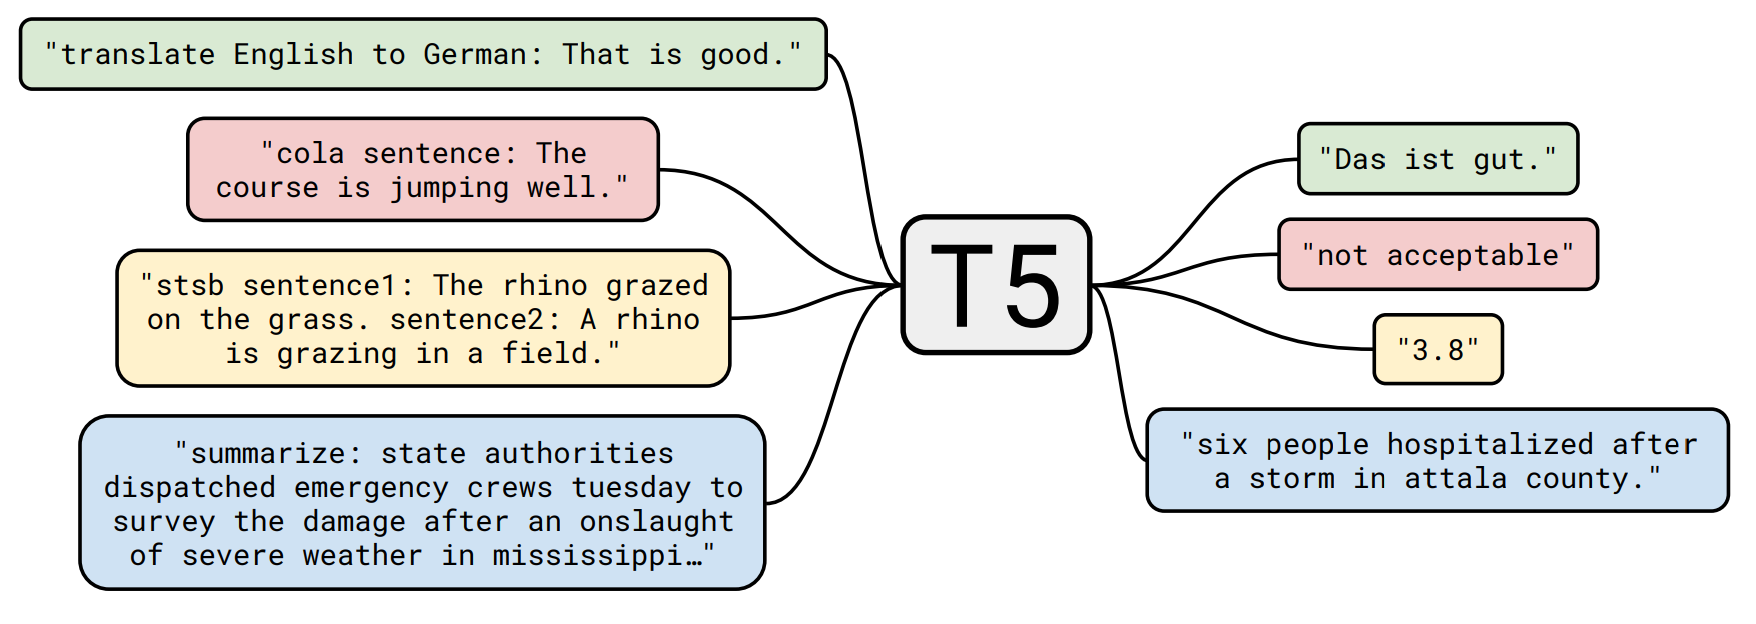
\includegraphics[width = 11cm]{figure/62-t5.png}\\ 
		\citebutton{Source: Raffel et al., 2020}{https://jmlr.org/papers/v21/20-074.html}
	\end{figure}
	
\textbf{Ingredients:}
	
\begin{itemize}
	\item \texttt{<task prefix>} for each task
	\item[] $\to$ Concatenation with the input
	\item Output label / score formatted as string
\end{itemize}
	
\vfill

\end{frame}

% ------------------------------------------------------------------------------

\begin{frame}{Text-to-Text Transfer Transformer}

\vfill

	\textbf{Short summary:}

	\begin{itemize}
		\item In short: T5 (bc of the five Ts)
		\item A complete encoder-decoder Transformer architecture
		\item[] \ques Why is this important?
		\item Relative positional embeddings
		\item All tasks reformulated as text-to-text tasks
		\item[] $\to$ Probably the most important innovation of this work
		\item From BERT-size $\times2$ (since enc-dec) up to 11B parameters
		\item Paradigm shift from \textit{Sequential Transfer Learning} towards true \textit{Multi-Task Learning}
	\end{itemize}
	
	\vspace{.5cm}

	\begin{center}
		\href{https://1.bp.blogspot.com/-o4oiOExxq1s/Xk26XPC3haI/AAAAAAAAFU8/NBlvOWB84L0PTYy9TzZBaLf6fwPGJTR0QCLcBGAsYHQ/s1600/image3.gif}{\textbf{\beamergotobutton{Nice Animation (similar to figure before)}}}
	\end{center}
	
\vfill

\end{frame}

% ------------------------------------------------------------------------------

\begin{frame}{input and output format}

\vfill

	\textbf{Input Side:}

	\begin{itemize}
		\item SentencePiece framework w/ WordPiece tokens
		\item Add task-specific (text) prefix to the original input
		\item Choice of the prefix: Hyperparameter!! 
		\item[$\to$] Changing this had limited impact
		\item[$\to$] No extensive experiments performed by the authors
	\end{itemize}
	
	\vspace{.5cm}

	\textbf{Output Side:}

	\begin{itemize}
		\item Output as a word or a piece of text (also numerical similarity scores)
		\item If output not present in set of potential alternatives, prediction considered as wrong (many other possible ways; this is not trivial)
	\end{itemize}
	
\vfill

\end{frame}

% ------------------------------------------------------------------------------

\begin{frame}{task prefix vs. prompting}

\vfill

	\textbf{Adding task-specific (text) prefix:}

	\begin{itemize}
		\item Add task-specific (text) prefix to the original input
		\item Model is fine-tuned on samples prepended with this prefix
		\item[$\to$] It learns to recognize what it is expected to do when encountering a specific prefix at test time
		\item[$\to$] Probably because of this: limited impact found by the authors
	\end{itemize}
	
	\vspace{.5cm}

	\textbf{Prompting:}

	\begin{itemize}
		\item Refers to just querying a trained w/o fine-tuning it (cf. next chapter)
		\item Paradigm of Few-/Zero-Shot Learning
		\item This is found to have a \textit{huge} impact on model performance
	\end{itemize}
	
\vfill

\end{frame}

% ------------------------------------------------------------------------------

\begin{frame}{architectural differences}

\vfill
	
	\textbf{Attention patterns (top) and Schematics of considered architectures (bottom)}
	
	\begin{figure}
		\centering
		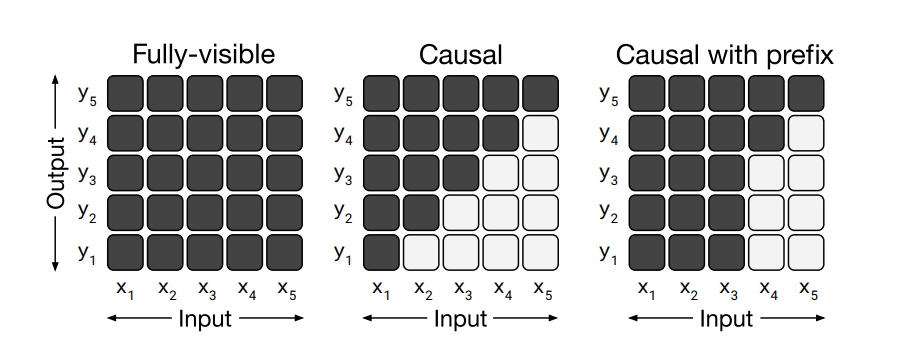
\includegraphics[width = 7.5cm]{figure/63-mask-patterns.png}\\ 
		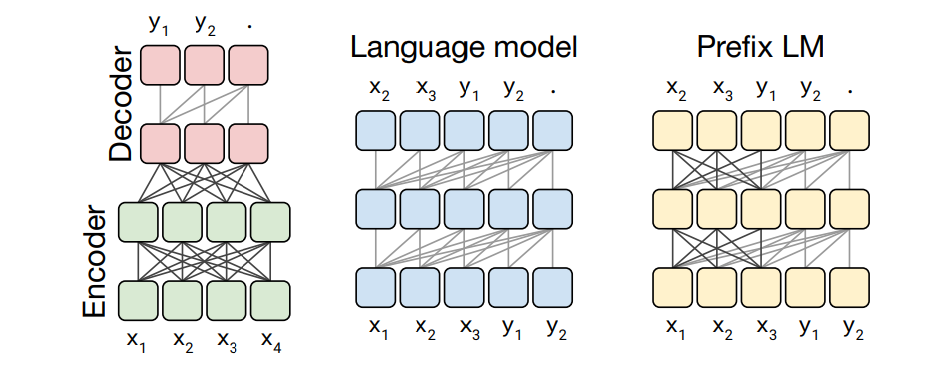
\includegraphics[width = 7.5cm]{figure/63-schematics.png}\\ 
		\citebutton{Source: Raffel et al., 2020}{https://jmlr.org/papers/v21/20-074.html}
	\end{figure}
	
\vfill

\end{frame}

% ------------------------------------------------------------------------------

\begin{frame}{pre-training objective}

\vfill
	
	\begin{figure}
		\centering
		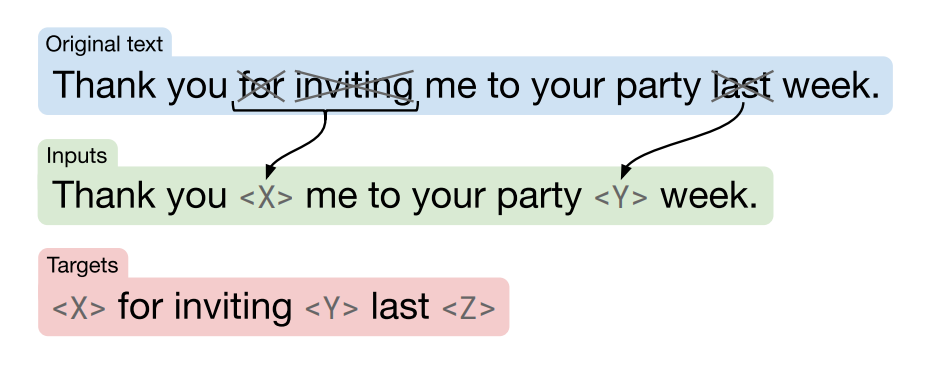
\includegraphics[width = 11cm]{figure/63-t5-span-pred.png}\\ 
		\citebutton{Source: Raffel et al., 2020}{https://jmlr.org/papers/v21/20-074.html}
	\end{figure}
	
	\begin{enumerate}
		\item Mark spans in input sequence for corruptions
		\item Replace tokens with sentinel tokens
		\item Predict sentinel tokens and replaced tokens
	\end{enumerate}
	
\vfill

\end{frame}

% ------------------------------------------------------------------------------

\begin{frame}{Pre-training objectives}

\vfill

	\begin{itemize}
		\item Authors experimented with different objectives
		\item Most of them rely in some way on MLM
	\end{itemize}
	
	\begin{figure}
		\centering
		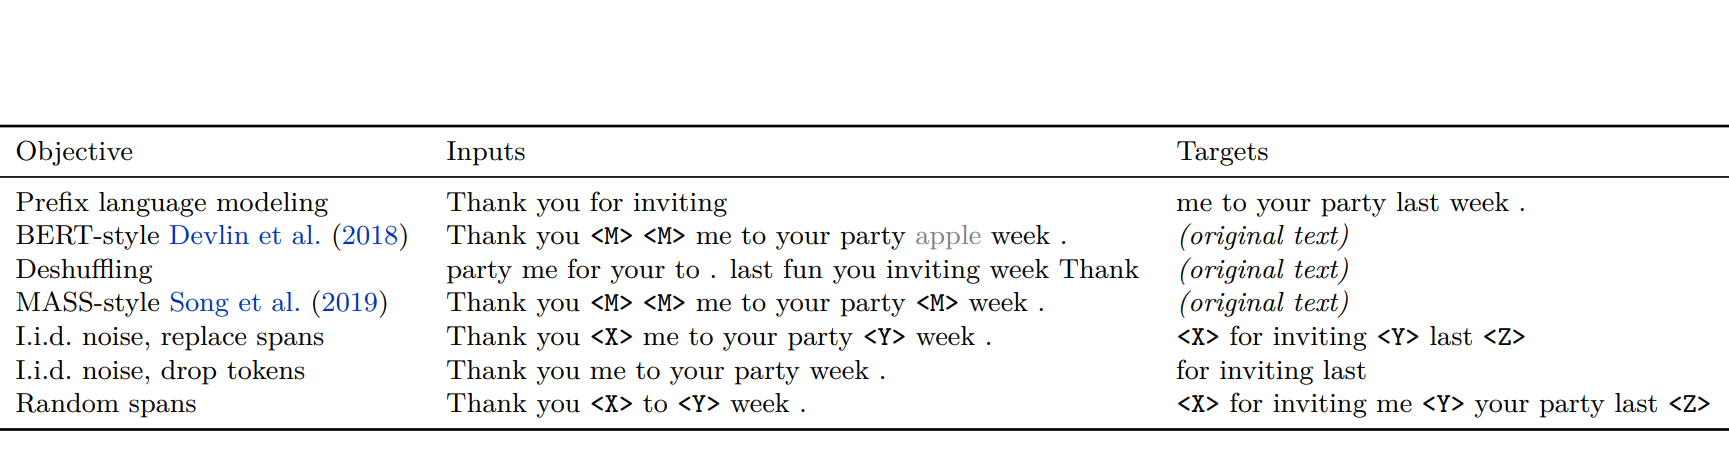
\includegraphics[width = 11cm]{figure/63-t5-objectives1.png}\\ 
		\citebutton{Source: Raffel et al., 2020}{https://jmlr.org/papers/v21/20-074.html}
	\end{figure}
	
\vfill

\end{frame}

% ------------------------------------------------------------------------------

\begin{frame}{Pre-training objectives}

\vfill

	\begin{figure}
		\centering
		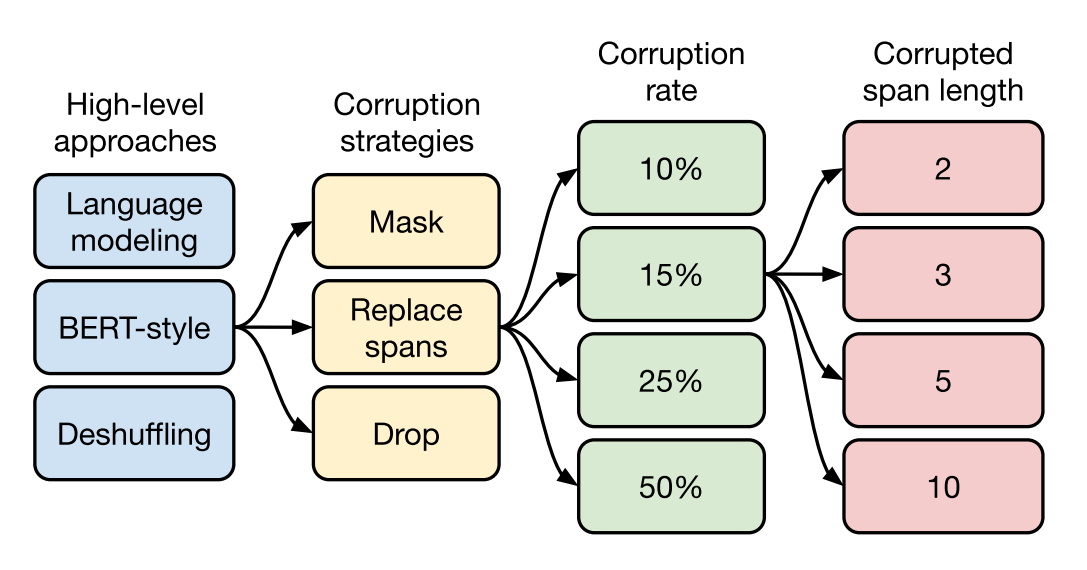
\includegraphics[width = 11cm]{figure/63-t5-objectives2.png}\\ 
		\citebutton{Source: Raffel et al., 2020}{https://jmlr.org/papers/v21/20-074.html}
	\end{figure}
	
\vfill

\end{frame}

% ------------------------------------------------------------------------------

\begin{frame}{The \textbf{C}olossal \textbf{C}lean \textbf{C}rawled \textbf{C}orpus (C4)}

\vfill

	\begin{itemize}
		\item Effort to measure the effect of quality, characteristics \& size of the pre-training resources
		\item Common Crawl as basis, careful cleaning and filtering for English language
		\item Orders of magnitude larger (750GB) compared to commonly used corpora 
	\end{itemize}
	
\vfill

\end{frame}

% ------------------------------------------------------------------------------

\begin{frame}{The \textbf{C}olossal \textbf{C}lean \textbf{C}rawled \textbf{C}orpus (C4)}

\vfill
	
	\textbf{Experiments (with respect to C4)}
	
	\begin{figure}
		\centering
		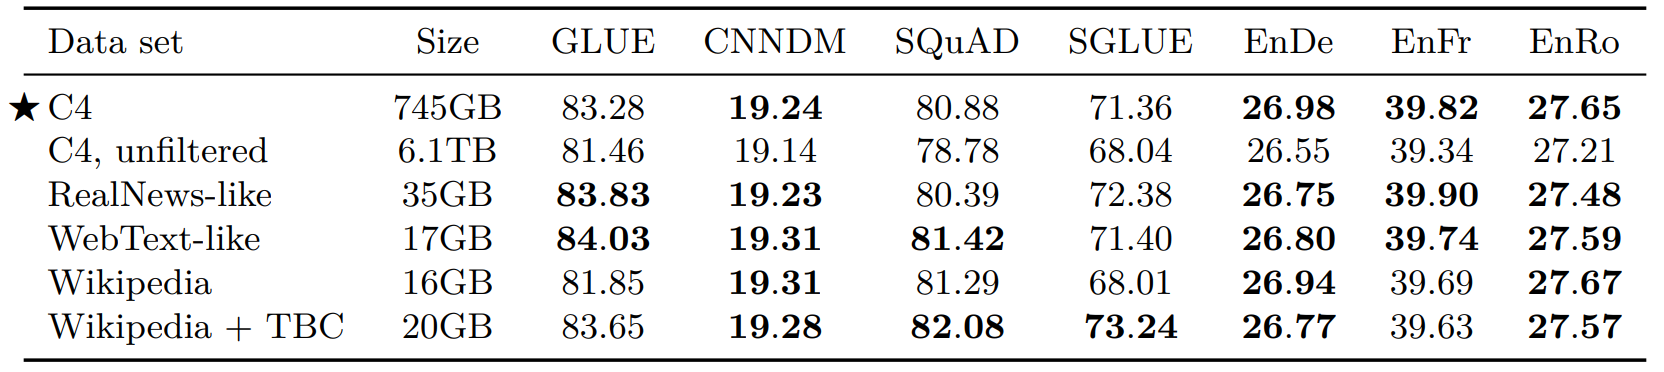
\includegraphics[width = 9cm]{figure/63-c4-characteristics.png}\\ 
		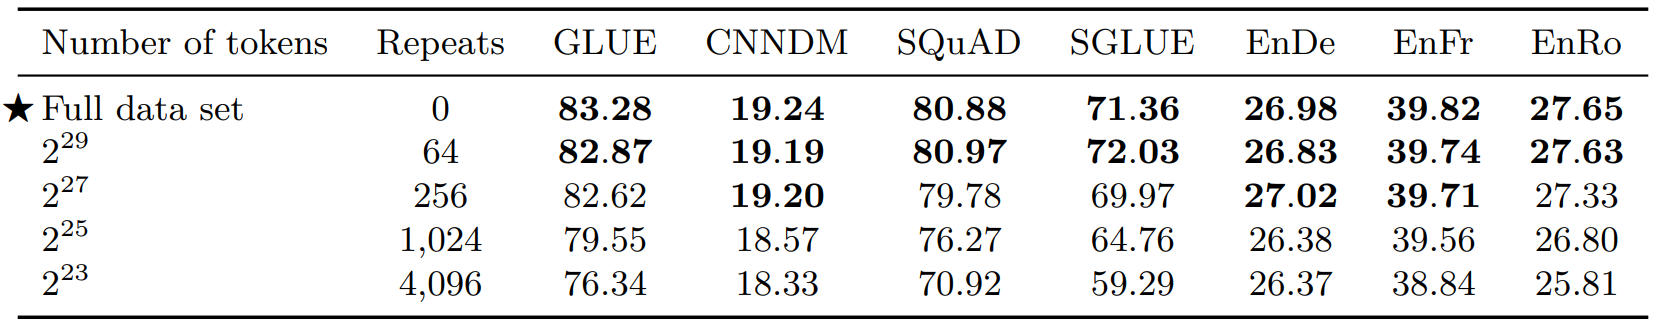
\includegraphics[width = 9cm]{figure/63-c4-size.png}\\ 
		\citebutton{Source: Raffel et al., 2020}{https://jmlr.org/papers/v21/20-074.html}
	\end{figure}
	
\vfill

\end{frame}

% ------------------------------------------------------------------------------

\begin{frame}{T5 - Exhaustive Experiments}

\vfill

	\textbf{Performed experiments with respect to ..}
	
	\begin{itemize}
		\item \textit{.. architecture, size \& objective}
		\item[$\to$] enc, dec, enc-dec
		\item[$\to$] Between 60M and 11B parameters
		\item \textit{.. details of the Denoising objective (which was found to work best)}
		\item \textit{.. fine-tuning methods}
		\item[$\to$] Adapter layers
		\item[$\to$] Gradual Unfreezing (cf. ULMFiT)
		\item \textit{.. Multi-task learning strategies}
		\item[$\to$] Examples-proportional mixing
		\item[$\to$] Temperature-scaled mixing
	\end{itemize}
	
\vfill

\end{frame}

% ------------------------------------------------------------------------------

\begin{frame}{Benchmark results}

\vfill

	\begin{figure}
		\centering
		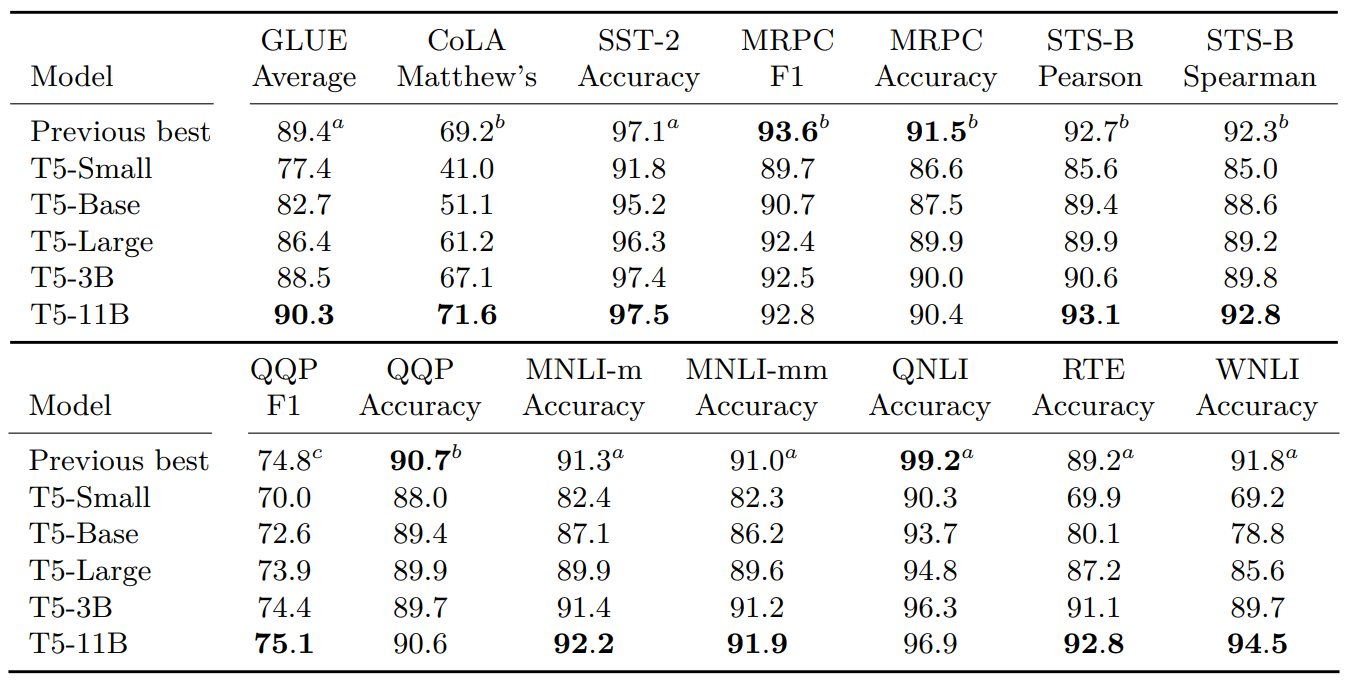
\includegraphics[width = 9cm]{figure/63-t5-glue.png}\\ 
		\citebutton{Source: Raffel et al., 2020}{https://jmlr.org/papers/v21/20-074.html}
	\end{figure}
	
\vfill

\end{frame}

% ------------------------------------------------------------------------------

\begin{frame}{Benchmark results}

\vfill

	\begin{figure}
		\centering
		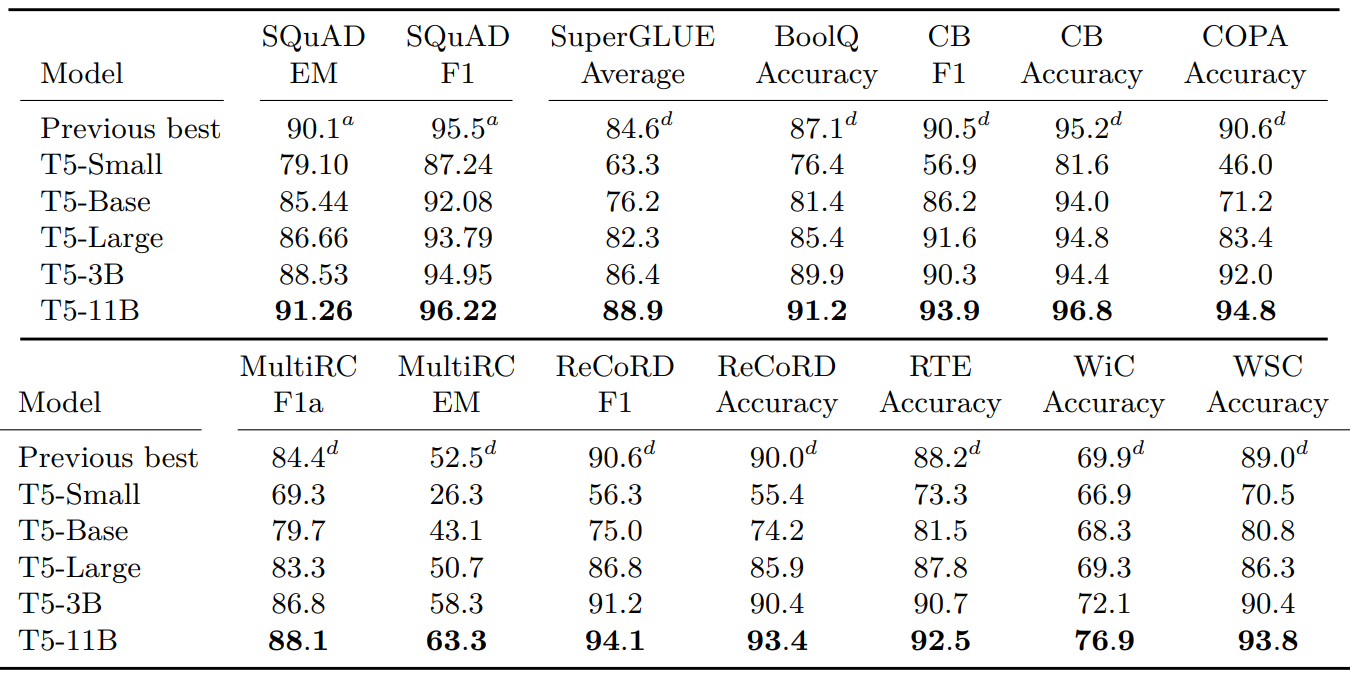
\includegraphics[width = 9cm]{figure/63-t5-squad-sglue.png}\\ 
		\citebutton{Source: Raffel et al., 2020}{https://jmlr.org/papers/v21/20-074.html}
	\end{figure}
	
\vfill

\end{frame}

% ------------------------------------------------------------------------------

\begin{frame}{Benchmark results}

\vfill

	\begin{figure}
		\centering
		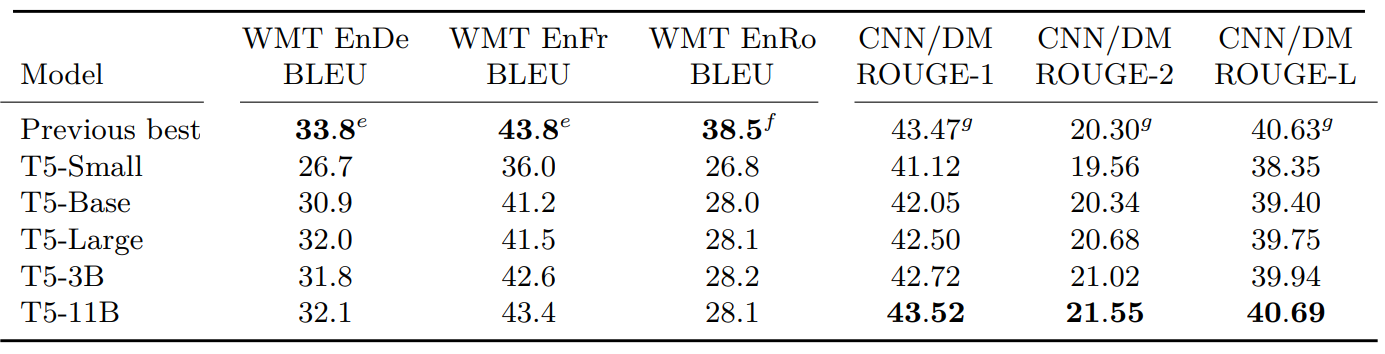
\includegraphics[width = 9cm]{figure/63-t5-mt.png}\\ 
		\citebutton{Source: Raffel et al., 2020}{https://jmlr.org/papers/v21/20-074.html}
	\end{figure}
	
\vfill

\end{frame}

% ------------------------------------------------------------------------------

\begin{frame}{T5 - Exhaustive Experiments}

\vfill
	
	\textbf{Conclusions}
	
	\begin{itemize}
		\item Encoder-decoder architecture works best in this "text-to-text" setting
		\item More data, larger models \& ensembling all boost the performance
			\begin{itemize}
				\item Larger models trained for fewer steps better than smaller models on more data
				\item Ensembling: Using same base pre-trained models worse than complete separate model ensembles
			\end{itemize}
		\item Different denoising objectives work similarly well
		\item Updating \textit{all} model parameters during fine-tuning works best (but expensive)
	\end{itemize}
	
\vfill

\end{frame}

% ------------------------------------------------------------------------------

\endlecture
\end{document}
